\documentclass{article}

\usepackage{graphicx}
\usepackage{tikz}
\usepackage{tikzsymbols}
\usetikzlibrary{calc,patterns,shapes.geometric}
\pagestyle{empty}
\usepackage[margin=0pt]{geometry}
\geometry{papersize={14in,12in}}

\def\centerarc[#1](#2)(#3:#4:#5){\draw[#1] ($(#2)+({#5*cos(#3)},{#5*sin(#3)})$) arc (#3:#4:#5);}

\begin{document}
	\begin{figure}
		\centering
		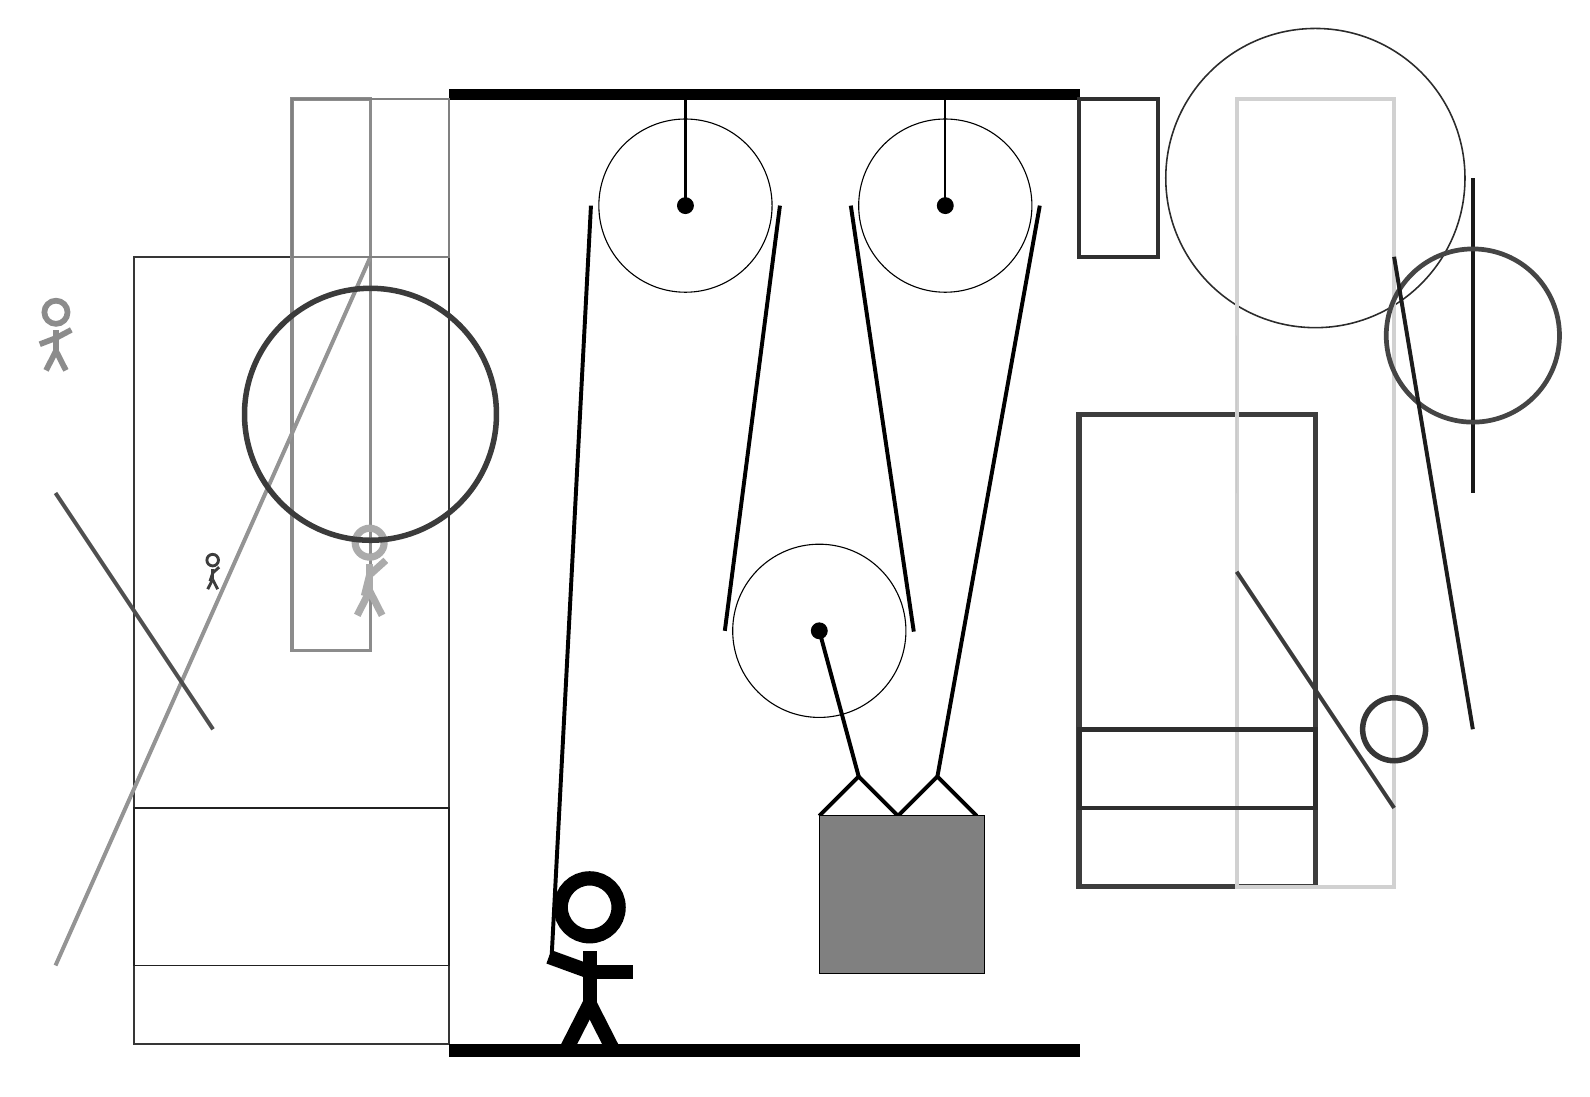
\begin{tikzpicture}
			%%%%% START %%%%%
			
			\draw[fill=black] (-2, 9) rectangle (6, 9.125);
			
			\draw (1, 7.65) circle (1.1);
			\draw[fill=black] (1, 7.65) circle (0.1);
			\draw[thick] (1, 7.65) -- (1, 9);
			
			\draw (4.3, 7.65) circle (1.1);
			\draw[fill=black] (4.3, 7.65) circle (0.1);
			\draw[thick] (4.3, 7.65) -- (4.3, 9);
			
			\draw (2.7, 2.25) circle (1.1);
			\draw[fill=black] (2.7, 2.25) circle (0.1);
			
			\draw[line width=0.5mm]  (2.7, -0.1) -- (3.2, 0.4) -- (3.7, -0.1) -- (4.2, 0.4) -- (4.7, -0.1);
			\draw[fill=black!50] (2.7, -0.1) rectangle (4.8, -2.1);
			
			\draw[line width=0.5mm](-0.7, -1.9) -- (-0.2, 7.65);
			\centerarc[line width=0.5mm](1, 7.65)(0:180:1.2000000000000002);
			\draw[line width=0.5mm](2.2, 7.65) -- (1.5, 2.25);
			\centerarc[line width=0.5mm](2.7, 2.25)(180:370:1.2000000000000002);
			\draw[line width=0.5mm] (3.9, 2.24) -- (3.1, 7.65);
			\centerarc[line width=0.5mm](4.3, 7.65)(0:180:1.2000000000000002);
			\draw[line width=0.5mm](4.2, 0.4) -- (5.5, 7.65);
			\draw[line width=0.5mm] (3.2, 0.4) -- (2.7, 2.25);
			
			\node at (-0.2, -2) {\Strichmaxerl[10][-20][0]};
			
			\draw[line width=0.7mm, color=black!76] (6, -1) rectangle (9, 5);
			
			\draw [line width=0.2mm, color=black!83](9, 8) circle (1.9);
			\draw[line width=0.3mm, color=black!79] (-2, -3) rectangle (-6, 7);
			\node[line width=0.4mm, color=black!45] at (-7, 6) {\Strichmaxerl[4][21][28]};
			
			\draw[line width=0.5mm, color=black!18] (8, -1) rectangle (10, 9);
			\draw[line width=0.2mm, color=black!87] (-2, -2) rectangle (-6, 0);
			
			\draw[line width=0.5mm, color=black!81] (6, 7) rectangle (7, 9);
			
			\draw[line width=0.5mm, color=black!45] (-3, 9) rectangle (-4, 2);
			\draw[line width=0.5mm, color=black!42](-3, 7) -- (-7, -2);
			
			\draw[line width=0.5mm, color=black!77](8, 3) -- (10, 0);
			\draw[line width=0.3mm, color=black!50] (-4, 7) rectangle (-2, 9);
			\draw [line width=0.7mm, color=black!79](10, 1) circle (0.4);
			\draw[line width=0.5mm, color=black!90](11, 8) -- (11, 4);
			
			\node[line width=0.7mm, color=black!33] at (-3, 3) {\Strichmaxerl[5][76][42]};
			\draw[line width=0.5mm, color=black!13](8, 0) -- (6, 0);
			\draw[line width=0.5mm, color=black!69](-5, 1) -- (-7, 4);
			
			\draw[line width=0.2mm, color=black!21] (8, 4) rectangle (8, 6);
			\node[line width=0.6mm, color=black!76] at (-5, 3) {\Strichmaxerl[2][72][42]};
			\draw [line width=0.6mm, color=black!73](11, 6) circle (1.1);
			\draw[line width=0.6mm, color=black!82] (6, 0) rectangle (9, 1);
			\draw [line width=0.7mm, color=black!77](-3, 5) circle (1.6);
			\draw[line width=0.5mm, color=black!89](10, 7) -- (11, 1);
			
			\draw[fill=black] (-2, -3) rectangle (6, -3.15);
			
			%%%%% END %%%%%
		\end{tikzpicture}
	\end{figure}	
\end{document}